\section{Javascript}
At its heart, javascript is a simple language. Its has however two very unconventional features that are not used in any other languages: \emph{this} and \emph{prototpye}s.  

\begin{itemize}
    \item Javascript does not have methods. It has properties that refer to functions.
    \item A function is an object. (Thats why every function has a \inlinecode{this}). Note that this means that there are executable objects.
\end{itemize}

 \paragraph{this}: every function implicitly gets a parameters named \inlinecode{this}, containing the context. 
\begin{lstlisting}
    function add (x, y) {
        console.log(this);
        return x + y;
    }
\end{lstlisting}
The context \inlinecode{this} can also be explicitly assigned.
\begin{lstlisting}
    const add3 = add.bind("michael", 2);
\end{lstlisting}
Note that this does not work for arrow-functions, which keep their once assigned context!


\paragraph{prototype}: Prototype-languages should really only achieve inheritance by copying objects. Javascript implements this badly, though, because it offers \emph{two} means of inheritance: object-copying and constructor-functions.
\begin{itemize}
    \item Instances 
        \begin{itemize}
            \item Every object has a \inlinecode{.__proto__}. 
            \item \inlinecode{.__proto__} contains the list of inherited props and methods and \emph{should} not be modified.
        \end{itemize}
    \item Constructing new objects
        \begin{itemize}
            \item With \inlinecode{Object.create}: passing \inlinecode{theObject.__proto__} and \inlinecode{theObject}'s instance-properties.
                \begin{itemize}
                    \item Calling \inlinecode{const vender = Object.create(bender); vender.name = 'Vender';} will give \inlinecode{vender} these properties: \inlinecode{bender.__proto__} and \inlinecode{bender}'s instance-properties;
                \end{itemize}
            \item With constructor functions: passing \inlinecode{TheFunction.prototype}
                \begin{itemize}
                    \item Functions are objects, so they, too, have a \inlinecode{.__proto__}
                    \item Additionally, functions have a \inlinecode{.prototype}. This is because any function may serve as a constructor, so they need this \inlinecode{.prototype}.
                    \item Even though not all functions are intended as constructors, js expects them to be that. So every function can be called with \inlinecode{new}. Doing this expects the function to do two things:
                        \begin{itemize}
                            \item it expects to have the function assign some things to its internal \inlinecode{this}. These assignments will be instance-properties.
                            \item it expects \inlinecode{TheFunction.prototype} to have a few props that are to be shared between all instances.
                        \end{itemize}
                    \item Contrary to \inlinecode{.__proto__}, \inlinecode{.prototype} may and should be modified.
                    \item So, calling \inlinecode{const bender = new Robot('Bender');} will give \inlinecode{bender} these properties: \inlinecode{Robot.prototype};
                \end{itemize}
            \item Funfact: \inlinecode{Object} is a constructor-function, which is why there is a \inlinecode{Object.prototype}. Indeed, calling \inlinecode{{name: 'Michael'}} is shorthand for \inlinecode{new Object({name: 'Michael'})} 
        \end{itemize}
\end{itemize}

\begin{lstlisting}
const Robot = function(name) {
    this.name = name;
}
Robot.prototype.sayHi = function() {
    return 'Hi from ' + this.name;
};
const bender = new Robot('Bender');
bender.sayHi();
Robot.prototype.sayHi = function() {
    return 'Bugger off from ' + this.name;
}
bender.sayHi();
\end{lstlisting}

\subsection{The js-runtime}
\begin{figure}[H] \label{js-runtime}
    \caption{\emph{Stack}: Todo's in the current frame. Makes calls to the \emph{Web-API}s. \emph{Queue}: From another thread the browser sends messages onto the queue. Some of these messages may have been triggered by the JS-stack calling for example a \inlinecode{setTimeout} Web-API call. They're handled FIFO.}
    \centering
    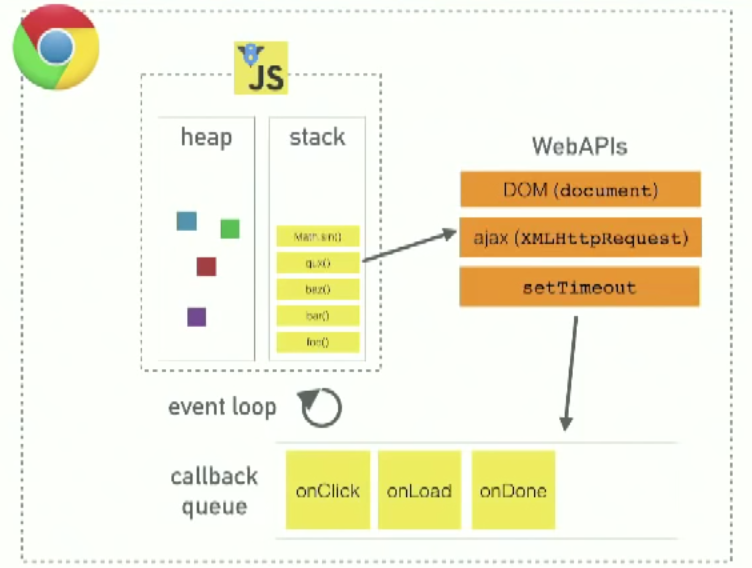
\includegraphics[width=0.75\textwidth]{images/js_event_loop.png}
\end{figure}

\subsection{Asynchronous programming}

Rxjs is a popular, stream based implementation of the observer-pattern.

\begin{lstlisting}
export interface Observer<T> {
    onNext: (val: T) => void,
    onCompleted: () => void,
    onError: (e: Error) => void
}


const nullObserver: Observer<any> = {
    onNext: (val: any) => {},
    onCompleted: () => {},
    onError: (e: Error) => {}
}


/**
 * Subscriptions are just handles to observers,
 * so that they can be unsubscribed if need be.
 */
export interface Subscription {
    unsubscribe: () => void;
}


export class SimpleSubscription<T> implements Subscription {
    constructor(
        private observer: Observer<T>
    ) {}

    unsubscribe () {
        // unsupscription == overwrite original observer
        this.observer = nullObserver;
    }
}


/**
 * 
 */
export class Observable<T> {

    constructor(
        private _subscribe: (observer: Observer<T>) => Subscription
    ) {}


    subscribe(downstreamObserver: Observer<T>): Subscription {
        return this._subscribe(downstreamObserver);
    }


    /**
     * List of static creational methods.
     * They each return new observables. 
     * Note that those new observables do not execute the _subscribe mehtod yet.
     * that method is only executed when subscribe is executed. 
     */

    static of<X>(args: X[]): Observable<X> {
        return new Observable<X>((downstreamObserver: Observer<X>) => {
            console.log(`executing subscription-body (returned from 'of' method)`)

            args.forEach(val => downstreamObserver.onNext(val));
            downstreamObserver.onCompleted();

            return new SimpleSubscription(downstreamObserver);
        })
    }


    static fromEvent(source: Element, event: string): Observable<Event> {
        return new Observable<Event>((downstreamObserver: Observer<Event>) => {
            console.log(`executing subscription-body (returned from 'fromEvent' method)`)

            const callback = (e: Event) => downstreamObserver.onNext(e);
            source.addEventListener(event, callback);
            return {
                unsubscribe: () => source.removeEventListener(event, callback)
            }
        });
    }

    /**
     * list of non-static creational mehtods.
     * They each return new observables.
     * Note that the subscribe methods are not called yet with this method.
     */

    map<Y>(mapFunc: (v: T) => Y): Observable<Y> {
        return new Observable<Y>((downstreamObserver: Observer<Y>) => {
            console.log(`executing subscription-body (returned from 'map' method)`)

            const mappingObserver: Observer<T> = {
                onNext: (val: T) => {
                    const y: Y = mapFunc(val);
                    downstreamObserver.onNext(y);
                },
                onCompleted: () => downstreamObserver.onCompleted(),
                onError: (e: Error) => downstreamObserver.onError(e)
            };

            return this.subscribe(mappingObserver);
        });
    }


    filter(filterFunc: (v: T) => boolean): Observable<T> {
        return new Observable<T>((downstreamObserver: Observer<T>) => {
            console.log(`executing subscription-body (returned from 'filter' method)`)

            const filteringObserver: Observer<T> = {
                onNext: (val: T) => {
                    if (filterFunc(val)) {
                        downstreamObserver.onNext(val);
                    }
                },
                onCompleted: () => downstreamObserver.onCompleted(),
                onError: (e: Error) => downstreamObserver.onError(e)
            };

            return this.subscribe(filteringObserver);
        });
    }


    take(nr: number): Observable<T> {
        return new Observable<T>((downstreamObserver: Observer<T>) => {
            console.log(`executing subscription-body (returned from 'take' method)`)

            let i = 0;
            const takingObserver: Observer<T> = {
                onNext: (val: T) => {
                    if (i < nr) {
                        downstreamObserver.onNext(val);
                        i += 1;
                    } else {
                        downstreamObserver.onCompleted();
                    }
                },
                onCompleted: () => downstreamObserver.onCompleted(),
                onError: (e: Error) => downstreamObserver.onError(e)
            };

            return this.subscribe(takingObserver);
        })
    }

}

const list$ = Observable.of([1, 2, 3, 4, 5, 6, 7, 8]);

const list2$ = list$.map((v) => v+1);

const list3$ = list2$.filter((v) => v % 2 === 1);

const list4$ = list3$.take(3);

list4$.subscribe({
  onNext: (val: number) => console.log(val),
  onCompleted: () => {}, 
  onError: () => {}
});
\end{lstlisting}

Zones allow you to wrap multpile, potentially asynchronous callframes in one common environment.

\begin{lstlisting}
interface ZoneSpec {
    name: string;
    props?: object;
    onFork?;
    onIntercept?;
    onInvoke?;
    onScheduleTask?;
    onInvokeTask?;
    onCancelTask?;
    onHasTask?;
}
    
class Zone {
    private static _current: Zone = new Zone(null, {name: 'Base'});
    private _parent: Zone;
    private zoneSpec: ZoneSpec;
    
    constructor(parent: Zone, zoneSpec: ZoneSpec) {
        this._parent = parent;
        this.zoneSpec = zoneSpec;
    }
    
    static get current() {
        return Zone._current;
    }
    
    get name() {
        return this.zoneSpec.name;
    }
    
    get parent() {
        return this._parent;
    }
    
    get(key: string) {
        return this.zoneSpec.props ? this.zoneSpec.props[key] : null;
    }
    
    fork(newZoneSpec: ZoneSpec) {
        for (const key in this.zoneSpec) {
        if (key != 'name') {
            if (!newZoneSpec[key]) {
            newZoneSpec[key] = this.zoneSpec[key];
            }
        }
        }
        return new Zone(Zone.current, newZoneSpec);
    }
    
    run(callback) {
        Zone._current = this;
        callback();
        Zone._current = this.parent;
    }
    
}


const _setTimeout = (callback, time) => {
const zoneOnCreateTime = Zone.current;
const wrappedCallback = () => {
    zoneOnCreateTime.run(callback);
};
setTimeout(wrappedCallback, time);
}


const zoneBC = Zone.current.fork({
name: 'BC',
props: {
    message: "Hi! You can only see me inside BC!"
}
});


function c() {
console.log("executing c in zone ", Zone.current.name);
console.log("Here's the message data: ", Zone.current.get('message'));
}

function b() {
console.log("executing b in zone ", Zone.current.name);
console.log("Here's the message data: ", Zone.current.get('message'));
_setTimeout(c, 2000);
// c();
}

function a() {
console.log("executing a in zone ", Zone.current.name);
console.log("Here's the message data: ", Zone.current.get('message'));
zoneBC.run(b);
}

a();
console.log("this is root, running in zone ", Zone.current.name);
\end{lstlisting}

\subsection{Module system}


\begin{table}[ht]
    \begin{tabularx}{1.2\textwidth}{XXXXXX}
        & CommonJs                                                            & NodeJs                                                                   & AMD                                                                              & UMD                                                           & ES2015 aka. ES6                                           \\
        used by         & formerly node                                                       & node                                                                     & requirejs                                                                        &                                                               &                                                           \\
        module-file     & \inlinecode{exports.area = (r) = PI * r * r;}                       & \inlinecode{module.exports = \{area: (r) = PI * r * r; \}}               & \inlinecode{define}                                                              & First tries AMD, then commonJs, then exports as global.       & \inlinecode{export const sqrt = Math.sqrt;}               \\
        user-file       & \inlinecode{const module = require('./module.js'); module.area(4);} & \inlinecode{const module = require('./module.js'); module.area(4);}      & \inlinecode{require, import, module}                                             &                                                               & \inlinecode{\{import \{ sqrt \} from 'module';\}}         \\
        loads modules   & synchronously                                                       & synchronously                                                            & asynchronously                                                                   &                                                               &                                                           \\
        implementations & webpack, browserify                                                 & node, webpack, browserify                                                & requirejs                                                                        &                                                               & webpack, babel                                            \\
        Notes           & Used to be a candidate for node, but now abandoned.                 &                                                                          & Does not work well with node (there is amdefine to help, but not ideal, either). &                                                               & Official JS standard, but so far not implemented in any browser or nodejs.
    \end{tabularx}
\end{table}

    

\subsubsection{Building with webpack}
My builder of choice is webpack. Basically, webpack makes ES6-import and -export work. There is some nice documentation \href{https://what-problem-does-it-solve.com/webpack/index.html}{here}.

paragraph{General concepts}: Some concepts and nomenclature.

\begin{itemize}
    \item Loaders vs Plugins: loaders work on the individual file-level, plugins work at the bundle- or chunk-level.
    \item compiling: compiling means transforming (eg.) ts-code to some (older version of) js.
    \item bundling: bundling takes compiled code and uses the import statements to create one large file.
\end{itemize}

\paragraph{Module-resolution}: Webpack can work with most module-types that javascript has to offer.

\begin{itemize}
    \item Javascript: webpack works fine with commonJs, nodeJs, and AMD, but will sometimes have problems with UMD.
        \begin{itemize}
            \item if a package.json has a \emph{module} entry, this field indicates that there is a ES6 version of the code. This will be loaded then.
            \item if it has a \emph{main} entry, that one leads to the entry-file of a (usually UMD) module.
            \item otherwise, you cannot import a whole module, but must load by filename.
        \end{itemize}
    \item Typescript: \inlinecode{ import { b } from "moduleB"; }. If in tsconfig the property \inlinecode{compilerOptions.module} is not \inlinecode{'AMD' | 'System' | 'ES2015'}, then a variation of the node-resolution is used:
        \begin{itemize}
            \item \inlinecode{'/node_modules/moduleB.ts'}
            \item \inlinecode{'/node_modules/moduleB.tsx'}
            \item \inlinecode{'/node_modules/moduleB.d.ts'}
            \item \inlinecode{'/node_modules/moduleB/package.json'}  (if it specifies a "types" property)
            \item \inlinecode{'/node_modules/@types/moduleB.d.ts'}
            \item \inlinecode{'/node_modules/moduleB/index.ts'}
            \item \inlinecode{'/node_modules/moduleB/index.tsx'}
            \item \inlinecode{'/node_modules/moduleB/index.d.ts'}
        \end{itemize}
    \item A note on Typescript's \inlinecode{import} and \inlinecode{require} statements: With TypeScript, \inlinecode{import} can be used if there is a declaration file for the module. If there isn't a declaration file, the TypeScript compiler doesn't know if the module exists, so you need to use \inlinecode{require} instead which lacks the compilation checking.
    \item Other languages: how to resolve other languages (ts, coffee, sass, shader, ...) is left over to loaders.
\end{itemize}

\paragraph{Shimming}: Webpack only loads a module when it sees it required at some point. This makes for smaller bundles, of course, but here is one problem this can cause. Say you have a dependency to jQuery and bootstrap. JQuery exposes \inlinecode{window.\$} as a global object. Bootstrap requires there to be a global \inlinecode{window.\$} object. However, since bootstrap just assumes that \inlinecode{window.\$} is there without ever calling \inlinecode{import}, webpack won't resolve the dependency and never include jQuery in the package. To avoid such problems, there is something called \emph{shimming}. 

\begin{lstlisting}
plugins: [
    new CopywebpackPlugin([ \{ from: path.resolve(__dirname, 'node_modules/cesium/Build/Cesium/Workers'), to: 'Workers' \} ]),
    new CopywebpackPlugin([ \{ from: path.resolve(__dirname, 'node_modules/cesium/Source/Assets'), to: 'Assets' \} ]),
    new CopywebpackPlugin([ \{ from: path.resolve(__dirname, 'node_modules/cesium/Source/Widgets'), to: 'Widgets' \} ]),
    new webpack.DefinePlugin(\{
        CESIUM_BASE_URL: JSON.stringify(''),
    \}),
    new webpack.ProvidePlugin(\{
        Cesium: 'cesium/Build/Cesium/Cesium'
    \})
],
\end{lstlisting}

The \inlinecode{ProviderPlugin} makes Cesium available to the global workspace. If you don't want this, you might want to instead use the \inlinecode{module.rules.imports-loader}.

\paragraph{Path-resolution}: When you ask to import a string that doesn't have a leading \inlinecode{./}, it tells Webpack: "Look for the file everywhere on my hard drive except the current directory". I'm not kidding. You can see the output desperately climbing up your directory hierarchy looking for a directory called \inlinecode{node_modules} in which it hopes to find index.js.
When you precede the module name with a \inlinecode{./}, it tells Webpack to look in the current directory for the file. So, the rule of thumb is: your code usually has a ./ and third-party libraries don't.

\paragraph{3rd party libs} d3 is a good example of a big library moving to the new ES6 module-syntax. d3 has many 3rd party libs that depend on and extend d3. As of D3 4.0, none of the D3 modules (formerly known as plugins) rely on a global d3 object. Each module is available either as a UMD bundle for use in Node or browsers, and as ES modules for use in bundlers and other modern JavaScript environments. Note that d3-plus hsa somehow still not managed to switch.

\paragraph{How webpack does it}
Webpack compiles this code:
\begin{lstlisting}
// helpers.ts
export function sayHi(name: string): string {
    return `Hi, ${name}!`;
}

// index.ts
import { sayHi } from "./helpers";
console.log(sayHi('Michael'));
\end{lstlisting}

to this code: 
\begin{lstlisting}
// self calling function
(function(modules) {
        // The module cache
        var installedModules = {};
    
        // The require function
        function __webpack_require__(moduleId) {
    
            // Check if module is in cache
            if(installedModules[moduleId]) {
                return installedModules[moduleId].exports;
            }
            // Create a new module (and put it into the cache)
            var module = installedModules[moduleId] = {
                i: moduleId,
                l: false,
                exports: {}
            };
    
            // Execute the module function
            modules[moduleId].call(module.exports, module, module.exports, __webpack_require__);
    
            // Flag the module as loaded
            module.l = true;
    
            // Return the exports of the module
            return module.exports;
        }
    
        // expose the modules object (__webpack_modules__)
        __webpack_require__.m = modules;
    
        // expose the module cache
        __webpack_require__.c = installedModules;
    
        // define getter function for harmony exports
        __webpack_require__.d = function(exports, name, getter) {
            if(!__webpack_require__.o(exports, name)) {
                Object.defineProperty(exports, name, { enumerable: true, get: getter });
            }
        };
    
        // define __esModule on exports
        __webpack_require__.r = function(exports) {
            if(typeof Symbol !== 'undefined' && Symbol.toStringTag) {
                Object.defineProperty(exports, Symbol.toStringTag, { value: 'Module' });
            }
            Object.defineProperty(exports, '__esModule', { value: true });
        };
    
        // create a fake namespace object
        // mode & 1: value is a module id, require it
        // mode & 2: merge all properties of value into the ns
        // mode & 4: return value when already ns object
        // mode & 8|1: behave like require
        __webpack_require__.t = function(value, mode) {
            if(mode & 1) value = __webpack_require__(value);
            if(mode & 8) return value;
            if((mode & 4) && typeof value === 'object' && value && value.__esModule) return value;
            var ns = Object.create(null);
            __webpack_require__.r(ns);
            Object.defineProperty(ns, 'default', { enumerable: true, value: value });
            if(mode & 2 && typeof value != 'string') for(var key in value) __webpack_require__.d(ns, key, function(key) { return value[key]; }.bind(null, key));
            return ns;
        };
    
        // getDefaultExport function for compatibility with non-harmony modules
        __webpack_require__.n = function(module) {
            var getter = module && module.__esModule ?
                function getDefault() { return module['default']; } :
                function getModuleExports() { return module; };
            __webpack_require__.d(getter, 'a', getter);
            return getter;
        };
    
        // Object.prototype.hasOwnProperty.call
        __webpack_require__.o = function(object, property) { return Object.prototype.hasOwnProperty.call(object, property); };
    
        // __webpack_public_path__
        __webpack_require__.p = "";
    
    
        // Load entry module and return exports
        return __webpack_require__(__webpack_require__.s = 0);
    })({
    
        // dependency
        "./src/dependency.ts": (function(module, __webpack_exports__, __webpack_require__) {
            function sayHi(name) {
                return "Hi, " + name + "!";
            }
            __webpack_require__.r(__webpack_exports__);
            __webpack_require__.d(__webpack_exports__, "sayHi", function() { return sayHi; })
        }),
    
        // script 
        "./src/index.ts": (function(module, __webpack_exports__, __webpack_require__) {
            __webpack_require__.r(__webpack_exports__);
            var _helpers__WEBPACK_IMPORTED_MODULE_0__ = __webpack_require__("./src/helpers.ts");
            console.log(Object(_helpers__WEBPACK_IMPORTED_MODULE_0__["sayHi"])('Michael'));
        })
});
\end{lstlisting}


\subsection{Promises, async-await and rxjs}
\inlinecode{async} - \inlinecode{await} lets you handle asynchronous code as if it was synchronous. 

\subsection{Webworkers: multithreading}


\subsection{WASM}
\begin{itemize}
    \item If wasm does not get a garbage-collector, 
        \begin{itemize}
            \item there will be no easy way for non-gc languages to run in wasm. They need to bring their own gc (or even runtime) with them (like c\# does now). 
            \item In that case, a situation like python + numy will probably evolve.
        \end{itemize}
    \item If wasm will not allow DOM-manipulation, 
        \begin{itemize}
            \item then there really is no point for non nummeric-focussed languages to be implemented in wasm.
            \item In that case, a situation like python + numy will probably evolve.
        \end{itemize}
    \item If, however, wasm will get a gc and allow DOM-manipulation, 
        \begin{itemize}
            \item Then python, ruby etc. will all develop angular-clones to run on the web. 
            \item However, given the large js-ecosystem, those will not kick in too mightily. 
        \end{itemize}
\end{itemize}


\section{CSS}

\subsection{Position}
\begin{itemize}
    \item \textbf{static}: the default
    \item \textbf{relative}: default + allows top, bottom, left and right
    \item \textbf{fixed}: relative to viewport
    \item \textbf{absolute}: relative to nearest positioned parent (positioned: anything but static)
    \item \textbf{sticky}: like fixed, but relative to container instead of viewport.
\end{itemize}

\subsection{Display}
Per default, divs are dispayed in blockstyle, while spans are displayed inlinestyle.
\begin{itemize}
    \item \textbf{block}
    \item \textbf{inline}
    \item \textbf{inline-block}: inline, but allows width, heigth, padding etc.
    \item \textbf{none}
    \item \textbf{table}
    \item \textbf{grid}
    \item \textbf{flex} see \ref{flexbox}
\end{itemize}

\subsubsection{Flexbox}\label{flexbox}

\section{Canvas}

\begin{table}[h]
    \begin{tabular}{@{}llll@{}}
    \toprule
    technology & use-case                    & programming style & libraries          \\ 
    \midrule
    canvas     & 3d, interactive, many items & procedural        & threejs, processing \\
    svg + css  & simple 2d graphics          & declarative       & d3                 \\ 
    \bottomrule
    \end{tabular}
\end{table}